\mcchap{Implementazione}{cap:cap4}
\section{Backend}
Il backend è la parte del sistema che si occupa dell'elaborazione dei dati e 
dell'interazione con il database. È responsabile della gestione delle 
richieste e delle risposte tra il frontend e il database.

Nel caso dell’Hotfix Response Center il backend è stato sviluppato 
utilizzando il framework Django, per Python. Django è stato utilizzato assieme 
alla libreria Django REST Framework per realizzare le API REST necessarie per 
la comunicazione tra frontend e backend.


\subsection{Api rest}
Le API REST (Representational State Transfer) sono un tipo di architettura 
software utilizzata per la progettazione e lo sviluppo di servizi web. 
Le API REST consentono alle applicazioni di comunicare tra loro e 
scambiare dati utilizzando i protocolli standard del web, come HTTP. 
Le API REST sono basate su un insieme di principi fondamentali. 
In primo luogo, utilizzano le risorse come concetto centrale, dove ogni 
risorsa rappresenta un'entità specifica (ad esempio, un oggetto, un 
utente, una transazione) e viene identificata da un URL univoco.

Le API REST utilizzano metodi HTTP come GET, POST, PUT, PATCH e DELETE 
per consentire alle applicazioni di accedere, creare, modificare o 
eliminare le risorse. Ad esempio, una richiesta HTTP GET a un'API REST 
può essere utilizzata per ottenere i dettagli di una risorsa, mentre una 
richiesta POST può essere utilizzata per creare una nuova risorsa.
Le API REST utilizzano anche la rappresentazione dei dati, di solito nel 
formato JSON o XML, per trasmettere le informazioni tra client e server. 
Questo permette una facile interoperabilità tra diverse piattaforme e 
linguaggi di programmazione.

Uno dei vantaggi delle API REST è la loro scalabilità e flessibilità. 
Le API REST sono state progettate per essere stateless, il che significa 
che ogni richiesta deve contenere tutte le informazioni necessarie per 
essere elaborata e non richiede lo stato persistente del server. Ciò 
consente una maggiore scalabilità del sistema e la possibilità di 
distribuire le risorse su più server. ~\cite{wiki:api_rest}\\


\subsection{Django}
\label{subsec:Django}
Django REST Framework, spesso abbreviato in DRF, è un framework 
open-source per lo sviluppo di API REST. Offre una serie di funzionalità 
che semplificano la creazione di API scalabili e ben documentate.
DRF si basa sui concetti fondamentali di Django, come il modello 
MVC (Model-View-Controller) e l'ORM (Object-Relational Mapping). 
Sfrutta la potenza di Django per fornire una struttura solida e coerente 
per la creazione di API REST. Con DRF, è possibile definire i modelli di 
dati utilizzando le classi Django (che verranno poi convertiti in tabelle).

Una delle caratteristiche chiave di DRF è la sua gestione avanzata della 
serializzazione dei dati. Questo consente di convertire facilmente gli 
oggetti Python in formati serializzati come JSON o XML e viceversa. 
DRF offre anche un sistema completo per la gestione dell'autenticazione 
e dell'autorizzazione delle API. È possibile configurare facilmente 
l'autenticazione basata su token, l'autenticazione OAuth2, l'autenticazione 
basata su sessione e altre modalità di autenticazione. Inoltre, supporta la 
definizione di permessi personalizzati per controllare l'accesso agli 
endpoint delle API in base a regole specifiche.

Un'altra caratteristica utile di DRF è la gestione delle route API. 
DRF offre un sistema di routing che consente di definire 
facilmente gli endpoint delle API e associarli alle corrispondenti view. 
Questo semplifica l'organizzazione delle API in base a risorse specifiche 
e facilita la creazione di endpoint RESTful standardizzati.
Infine, DRF include un modulo di documentazione automatica che genera 
automaticamente la documentazione delle API basandosi sulle definizioni 
delle API e dei serializer. Questo rende più semplice per gli sviluppatori 
e gli utenti delle API comprendere e utilizzare correttamente le risorse 
fornite dall'applicazione. ~\cite{wiki:django}\\


\subsection{Esempio}
I seguenti pezzi di codice illustrano in Django la realizzazione di 
un'API REST per la gestione delle campagne all'interno del backend.
In particolare, l'esempio illustra come definire un modello di dati per una 
campagna, creare URL per gestire le richieste relative alle campagne, definire 
una vista che si occupa di recuperare e creare campagne utilizzando il modello 
e serializzare i dati della campagna utilizzando un serializer.

\lstinputlisting[style=custompython, language=Python]{code/django.py}

Nel file models.py viene definita la classe Campaign che estende la classe 
models.Model. Questa classe rappresenta il modello di dati per una campagna e 
contiene tutti i campi definiti nel paragrafo ~\ref{subsec:Definizioni delle tabelle} 
relativo alla definizione delle tabelle. 
Ogni campo definisce il tipo di dati che può contenere e le 
eventuali opzioni di configurazione. 

Nel file views.py viene definita la classe CampaignListCreateAPIView che 
gestisce le richieste relative alle campagne. La variabile queryset definisce 
l'insieme di dati su cui operare, in questo caso tutte le campagne ordinate per 
l'ID. Vengono anche specificati i  filtri e l’ordinamento da utilizzare. 
La variabile serializer\_class definisce la classe del serializer da utilizzare 
per la serializzazione dei dati in JSON. 
Questa vista estende la classe generics.ListCreateAPIView 
fornita da Django REST Framework e fornisce funzionalità per visualizzare 
l'elenco delle campagne e creare una nuova campagna.

Nel file serializers.py viene definita la classe CampaignSerializer che gestisce 
la serializzazione dei dati della campagna. La classe Meta all'interno del 
serializer specifica il modello di riferimento (Campaign), i campi da includere 
nella serializzazione ('\_\_all\_\_' indica tutti i campi del modello) e i campi di 
sola lettura che non possono essere modificati.

Nel file urls.py viene definito il percorso delle API per gestire le richieste 
relative alle campagne. In particolare, quando viene inviata una richiesta all'endpoint 
/campaigns/, viene utilizzata la classe CampaignListCreateAPIView come vista 
per gestire la richiesta.\\

Facendo richieste di HTTP GET sull’endpoint /campaigns/ verrà fornito l’elenco 
delle campagne inserite nel database. Sarà possibile utilizzare i filtri 
come queryparams della richiesta per 
ricercare tra tutte le campagne solo quelle desiderate. Le informazioni saranno 
restituite in formato JSON con i campi definiti nel serializer.

Facendo invece una richiesta di HTTP POST sullo stesso endpoint sarà possibile 
creare una nuova campagna. Le informazioni della nuova campagna andranno 
inserite nel body della richiesta.
Per entrambe le richieste dovrà essere fornito il token di autenticazione per 
verificare l’identità e le autorizzazioni dell’utente che sta utilizzando i 
servizi.


\section{Frontend}
Il frontend è la parte dell’applicazione che interagisce direttamente con 
l’operatore. È responsabile della presentazione dei dati consentendo agli 
utenti di visualizzare e interagire con il contenuto dell'applicazione web.\\

Nel contesto dello sviluppo web, il frontend si riferisce alla combinazione 
di tecnologie, linguaggi di programmazione e strumenti utilizzati per creare 
l'interfaccia utente di un'applicazione web. Ciò include l'utilizzo di HTML 
(Hypertext Markup Language) per definire la struttura e il contenuto della 
pagina, CSS (Cascading Style Sheets) per definire il layout e l'aspetto 
visivo della pagina, e JavaScript per aggiungere interattività e funzionalità 
dinamiche.

In questo caso per lo sviluppo dell’interfaccia frontend si è deciso di 
utilizzare il framework Vue.js per semplificare lo sviluppo e migliorare 
l'efficienza di programmazione.

\subsection{Vue.js}
Vue.js è un framework JavaScript open-source progressivo utilizzato per la creazione di 
interfacce utente dinamiche e reattive. È incentrato sulla creazione di 
applicazioni web a pagina singola (Single-Page Applications) e si concentra 
sulla visualizzazione dei dati e sulla gestione dello stato dell'applicazione.

Le caratteristiche chiave di Vue.js includono la reattività dei componenti, 
la gestione dichiarativa degli elementi del documento HTML, un sistema di 
componenti componibile e la capacità di gestire lo stato dell'applicazione in 
modo efficiente. Vue.js offre anche una vasta gamma di strumenti e librerie di 
supporto, oltre a una comunità attiva che contribuisce allo sviluppo e 
all'evoluzione del framework.

Con la sua sintassi intuitiva e la facilità d'uso, Vue.js è diventato popolare 
tra gli sviluppatori per la creazione di interfacce utente complesse, ma 
mantenendo una curva di apprendimento accessibile. È ampiamente utilizzato per 
la creazione di applicazioni web moderne e reattive, fornendo un'esperienza 
utente ottimizzata e una manutenzione semplificata del codice. 
~\cite{wiki:vuejs}\\


\section{Interfaccia utente ed esempio utilizzo}
Per accedere al pannello di controllo dell’Hotfix Response Center, gli utenti 
possono visitare la pagina web privata tramite il proprio browser. 
Una volta effettuato l'accesso al portale, verrà visualizzato un elenco delle 
campagne già a sistema.\\

Per vedere i dettagli delle campagne precedentemente create basterà fare click 
sulla riga corrispondente. Invece, per creare una nuova campagna, gli utenti 
possono fare click sul bottone “Crea una nuova campagna” posizionato nell'angolo 
in alto a destra dell’interfaccia.

\begin{figure}[H]
\begin{flushright}
    \centering
    \frame{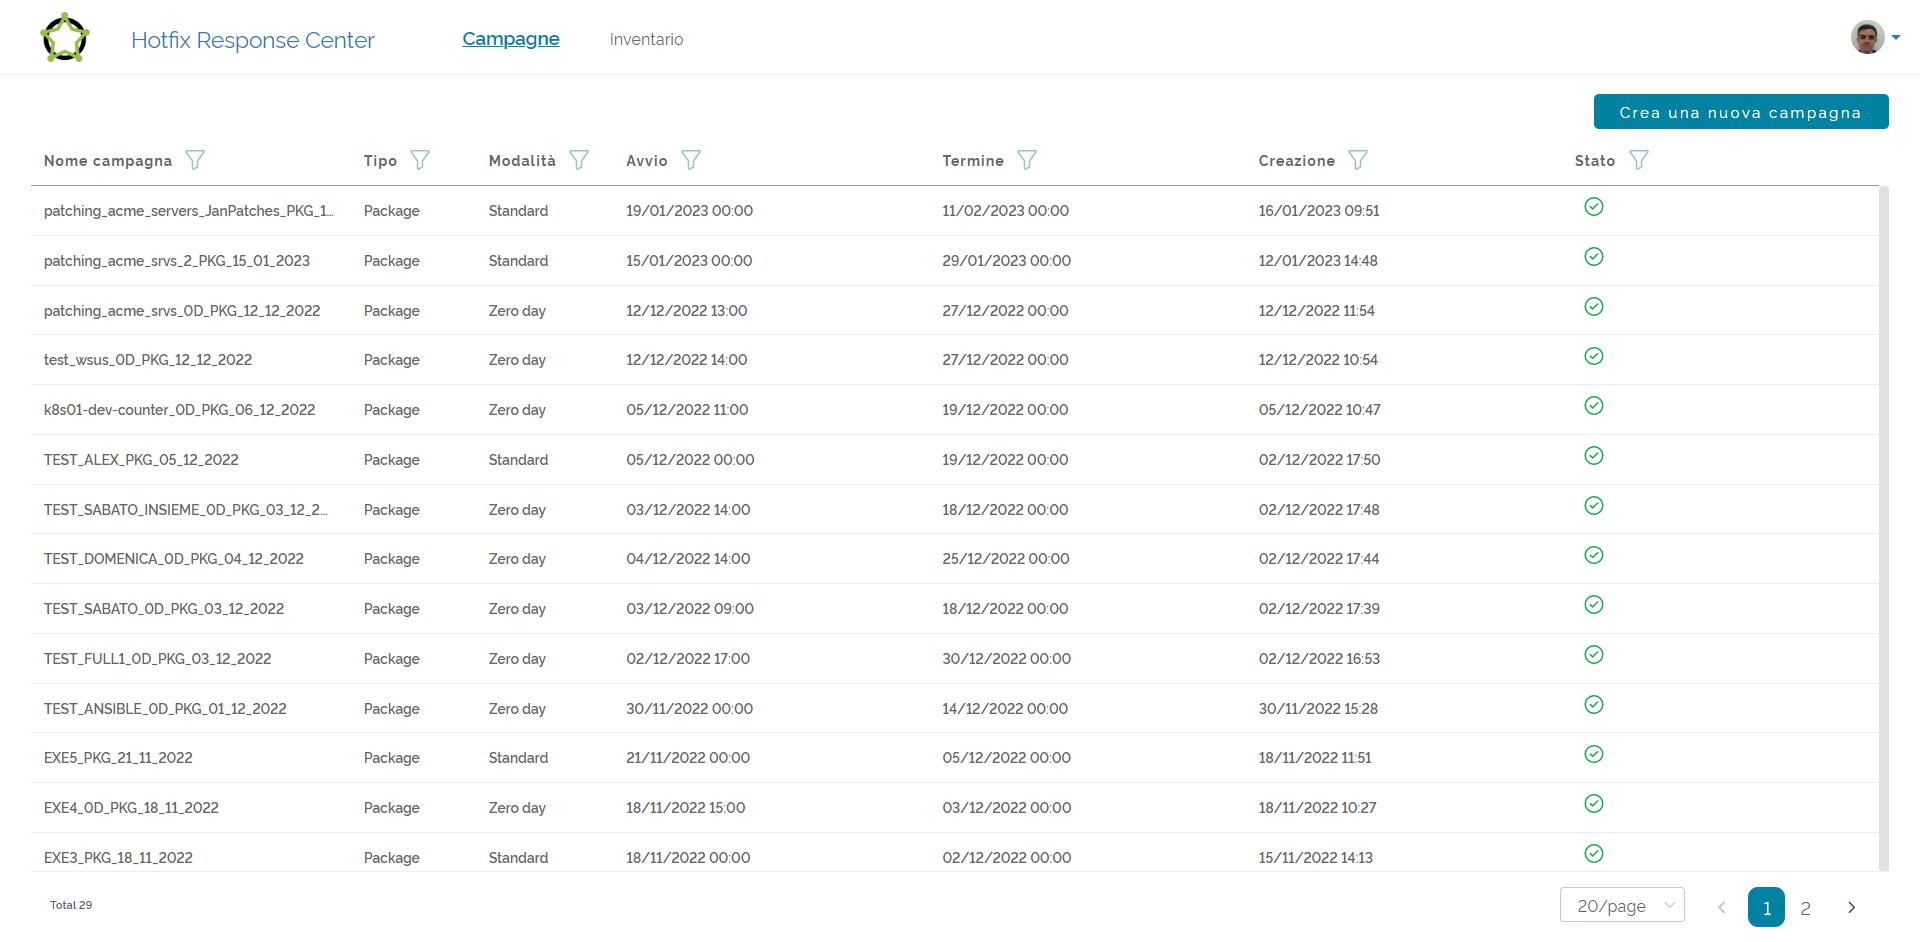
\includegraphics[width=0.98\textwidth]{imgs/ui/1_list_campaign.png}}
    \caption{Pagina principale, elenco delle campagne}
    \label{fig:Elenco delle campagne}
\end{flushright}
\end{figure}

Una volta che l'utente schiaccia il bottone per creare una nuova campagna, Vue.js 
esegue l'azione di click e carica dinamicamente la pagina specifica dedicata alla 
creazione della campagna. 

Questa pagina offre all'utente un'interfaccia intuitiva per inserire tutte 
le informazioni necessarie per avviare il processo di creazione 
della campagna. Attraverso questa pagina, l'utente può fornire le informazioni di base, 
come il nome della campagna, la modalità di esecuzione e le date di inizio e di 
fine.\\

Nella pagine successive verranno mostrate le schermate relative alla creazione di 
una campagna di aggiornamento su tutti i Windows Server di un cliente, per installare
un aggiornamento cumulativo rilasciato da Windows con identificativo KB5014850 che
serve a risolvere delle vulnerabilità di sistema.

\begin{figure}[H]
\begin{flushright}
    \centering
    \frame{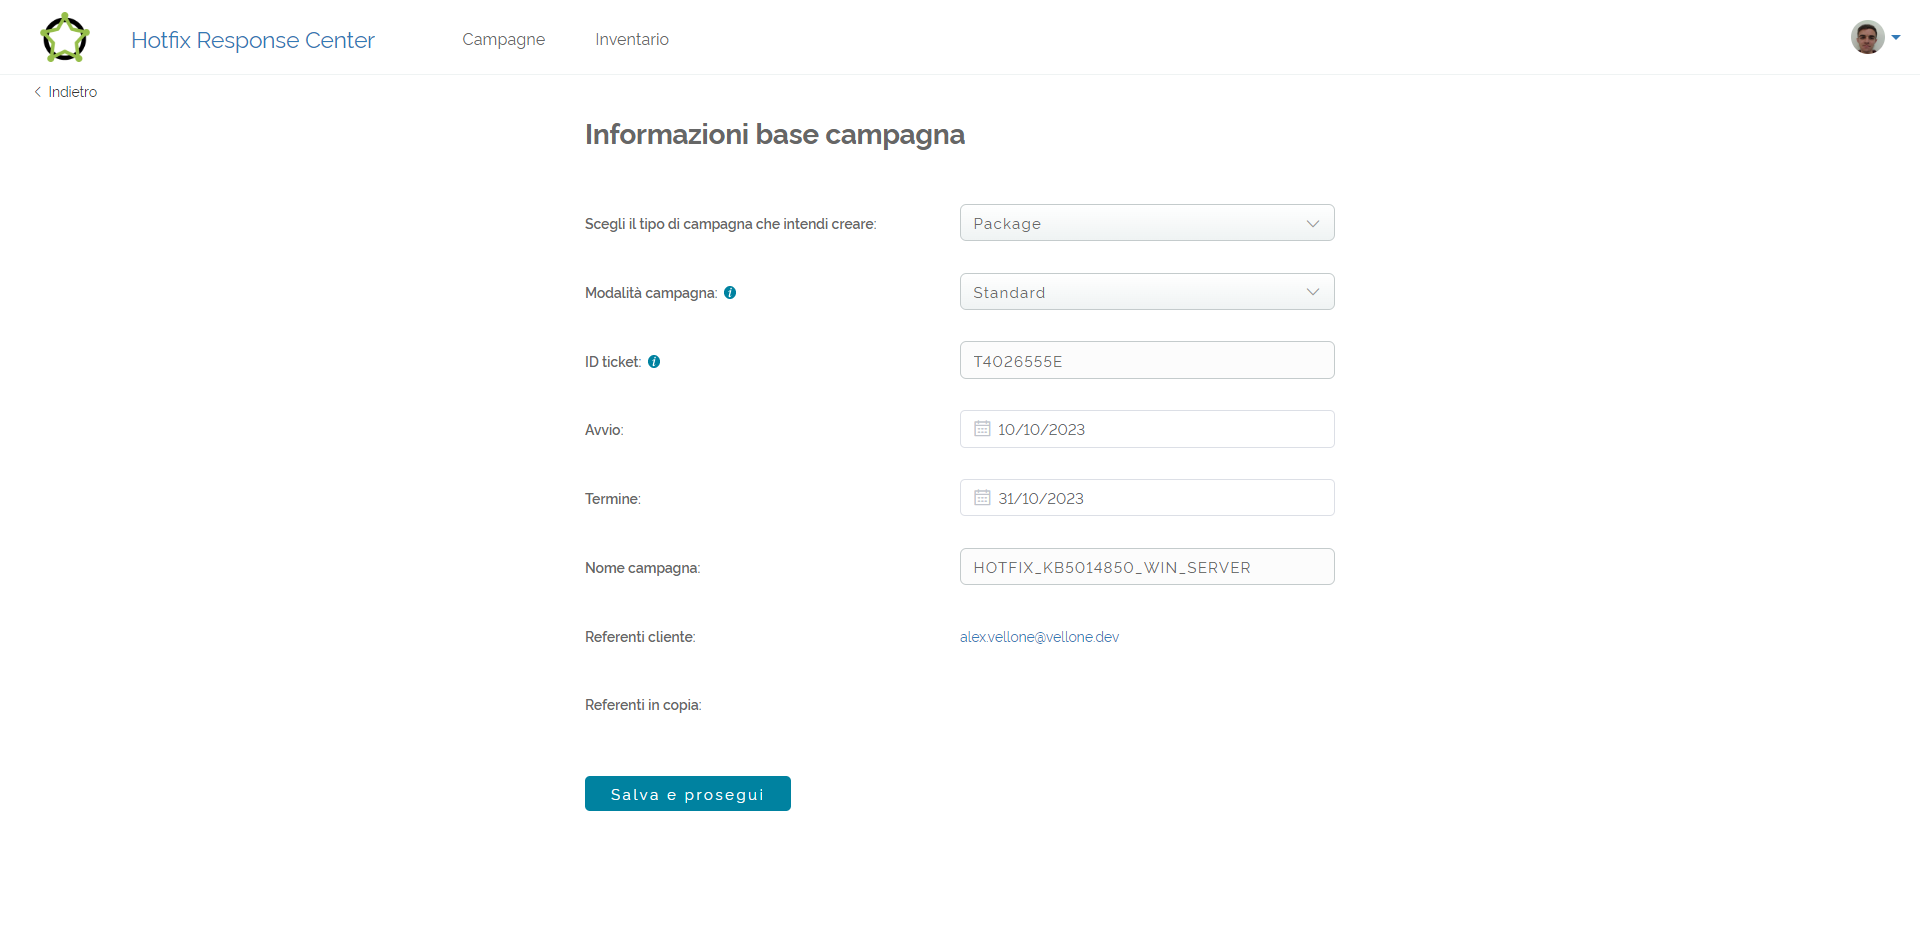
\includegraphics[width=0.95\textwidth]{imgs/ui/2_new_campagin.png}}
    \caption{Creazione di una nuova campagna}
    \label{fig:Creazione di una nuova campagna}
\end{flushright}
\end{figure}

Al click del bottone “Salva e prosegui” verrà eseguito il codice JavaScript per 
fare una chiamata POST alle API del backend con la quale verranno passate tutte le 
informazioni inserite dell’utente e verrà salvata la campagna all’interno del 
database.

Successivamente verrà mostrata la schermata per selezionare i server impattati 
dalla vulnerabilità. Da questa schermata è possibile utilizzare i filtri per 
selezionare rapidamente solo i server che si vogliono aggiornare.

\begin{figure}[H]
\begin{flushright}
    \centering
    \frame{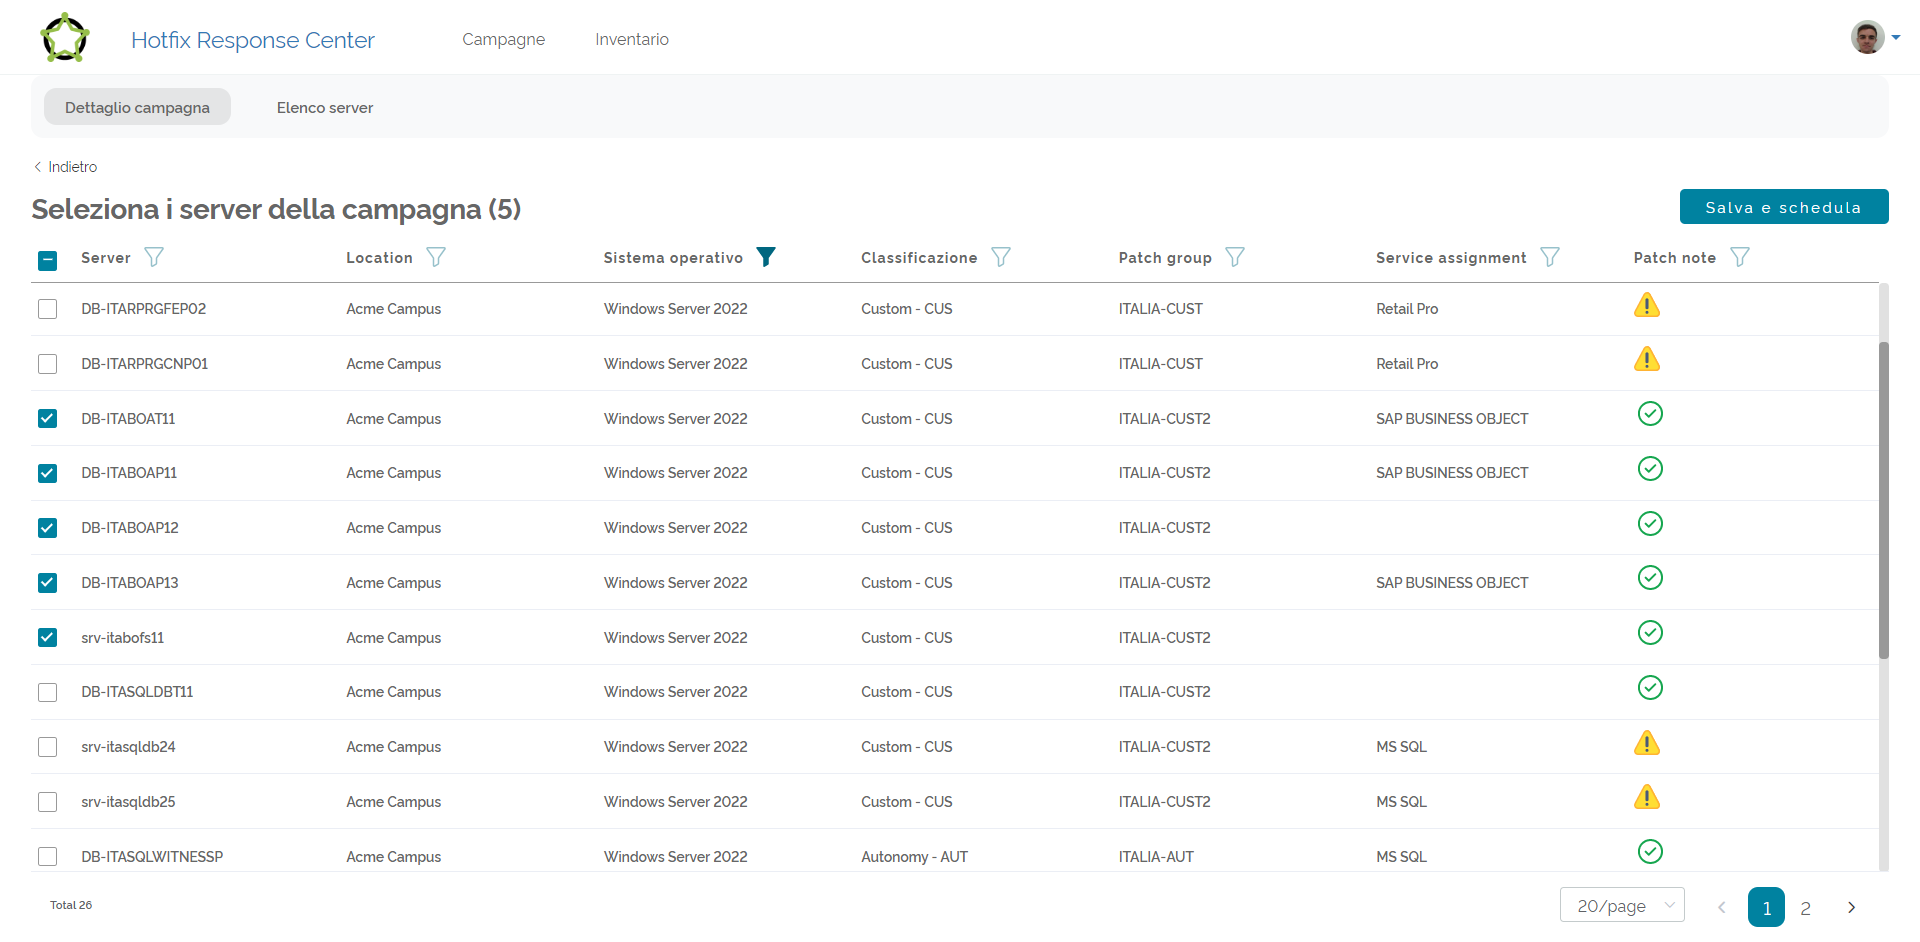
\includegraphics[width=0.95\textwidth]{imgs/ui/3_add_server.png}}
    \caption{Selezione elenco dei server impattati dalla vulnerabilità}
    \label{fig:Selezione elenco dei server impattati dalla vulnerabilità}
\end{flushright}
\end{figure}

Dopo aver selezionato tutti i server impattati sarà sufficiente fare click sul 
bottone “Salva e schedula” per inviare l’elenco dei server al backend, sempre 
tramite le API REST. 
Il backend avvierà a questo punto l’algoritmo di schedulazione per trovare uno
slot di manutenzione adatto per l'aggiornamento di tutti i server.

\begin{figure}[H]
\begin{flushright}
    \centering
    \frame{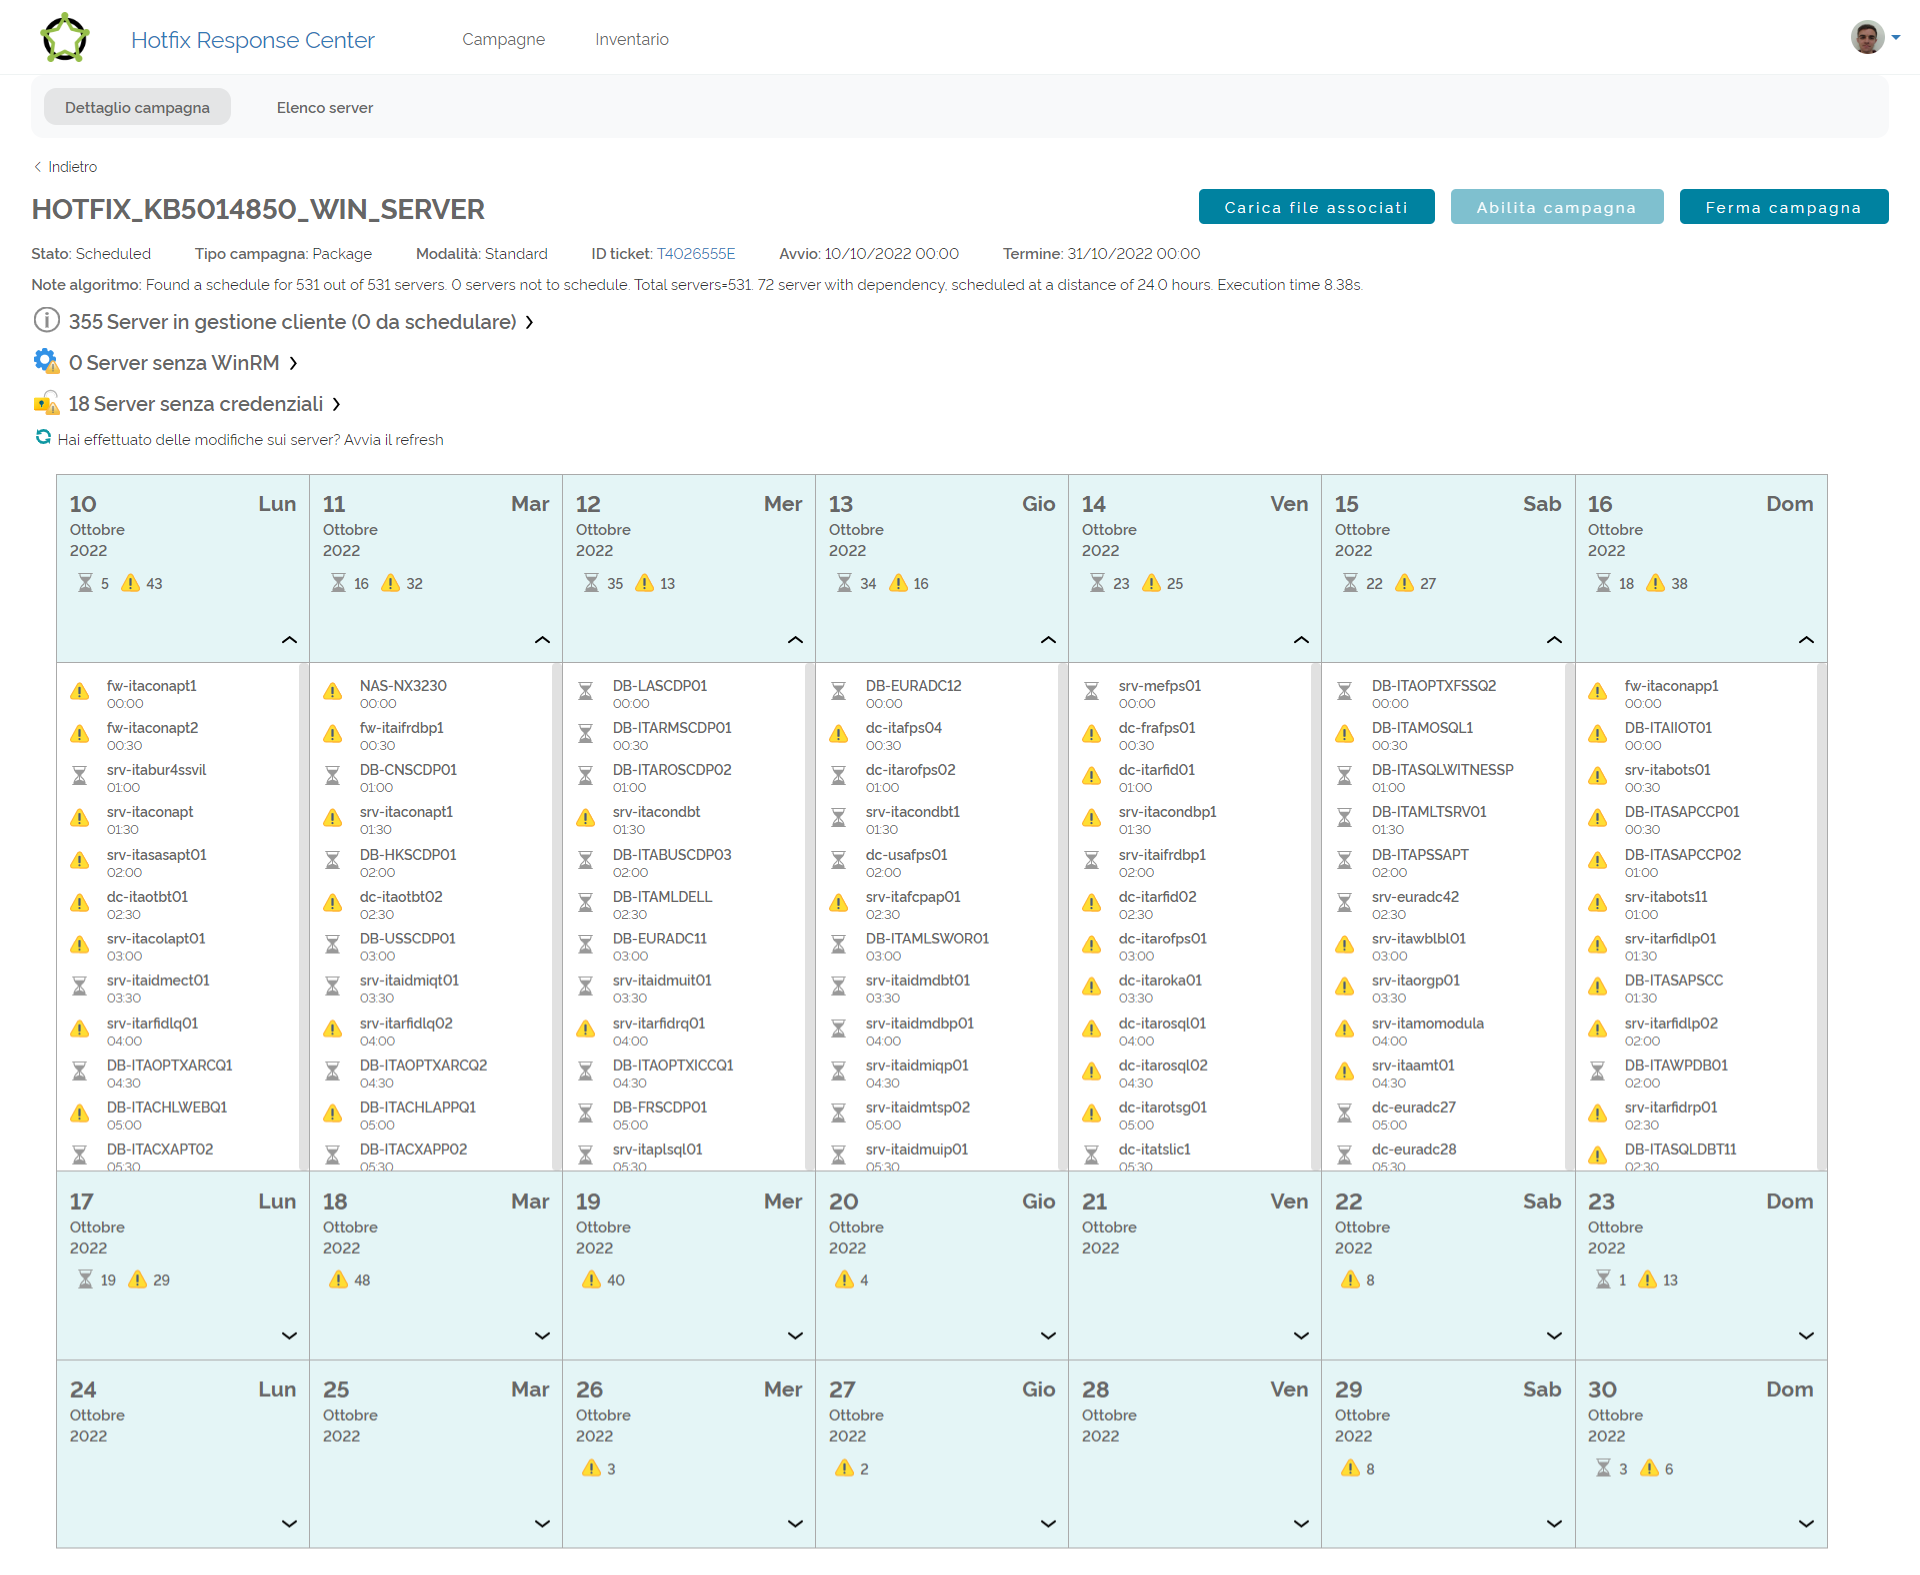
\includegraphics[width=0.98\textwidth]{imgs/ui/4_calendar.png}}
    \caption{Calendario della campagna}
    \label{fig:Calendario della campagna}
\end{flushright}
\end{figure}

Nella campagna selezionata sono stati inclusi 531 server, tutti pianificati con 
successo rispettando le rispettive finestre di manutenzione. Di questi, 72 sono 
stati considerati dipendenze e sono stati schedulati garantendo una separazione 
di 24 ore rispetto ai server di riferimento.

Per tutti i server della campagna è disponibile WinRM che consente quindi 
l'esecuzione automatica e remota degli aggiornamenti. Tuttavia, per 355 server 
è necessaria l'approvazione del cliente prima di procedere, mentre per 18 
server mancano le credenziali di connessione remota. Queste eccezioni sono 
segnalate nel calendario tramite un'icona di avviso, mentre per gli altri server 
gli aggiornamenti automatici partiranno nel rispettivo orario prestabilito.
I server con gli avvisi dovranno essere approvati per tempo dal cliente e 
l'operatore avrà del tempo per sistemare i problemi di credenziali sui 18 server.\\

Il calendario mostra un riepilogo, per ciascun giorno della campagna, 
consentendo di visualizzare i server schedulati nella giornata espandendo la 
settimana tramite un pulsante con una freccia verso il basso.

La pianificazione evidenzia in modo accurato come l'algoritmo abbia schedulato 
numerosi server nella prima settimana, riempiendo quasi completamente i 48 slot 
giornalieri disponibili. Nella terza settimana sono stati pianificati i server 
che presentano una programmazione più complessa a causa delle restrizioni imposte 
dalle finestre di manutenzione.\\

Prima dell'avvio della campagna, è necessario caricare i file di aggiornamento. 
In particolare, si mira a risolvere un gruppo di vulnerabilità nei sistemi 
operativi Windows Server utilizzando l'aggiornamento di sicurezza cumulativo 
con identificativo KB5014850, fornito da Microsoft.

Cliccando sul pulsante “Carica file associati”, si accede alla schermata dedicata 
al caricamento delle patch di sicurezza.

\begin{figure}[H]
\begin{flushright}
    \centering
    \frame{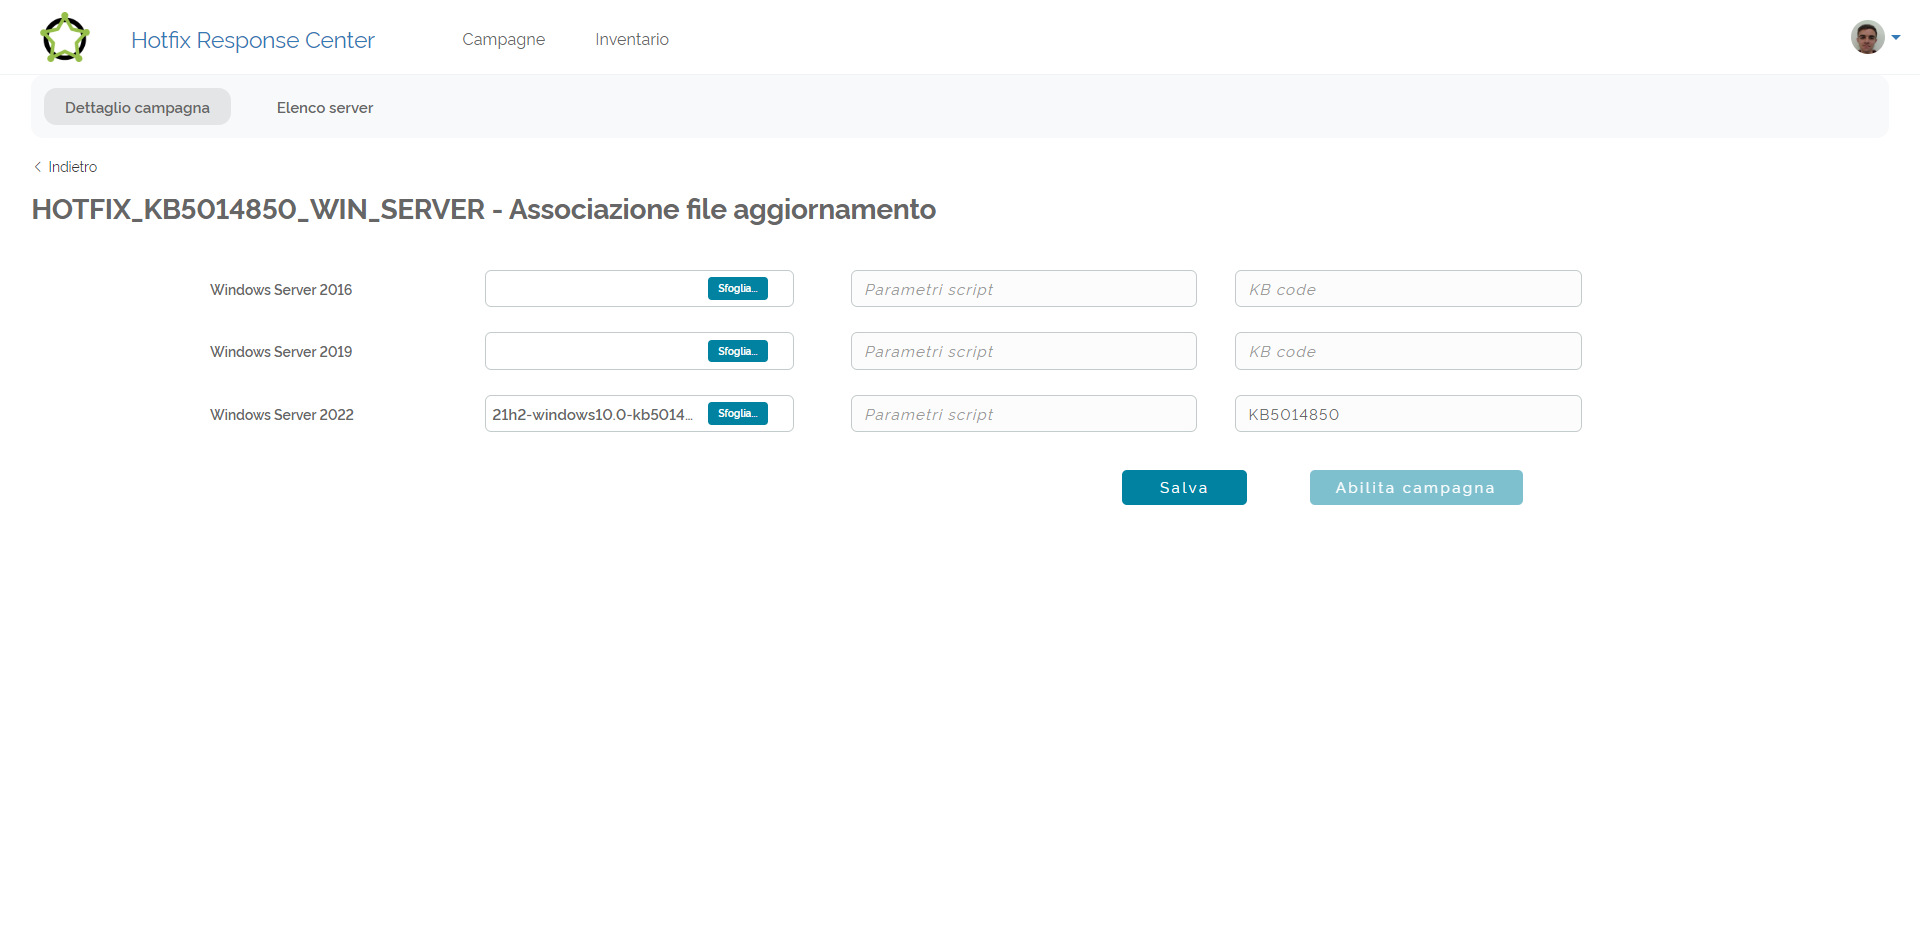
\includegraphics[width=0.98\textwidth]{imgs/ui/5_upload_files.png}}
    \caption{Upload dei file di aggiornamento}
    \label{fig:Upload dei file di aggiornamento}
\end{flushright}
\end{figure}

Considerando i 531 server selezionati, si rilevano tre diversi sistemi operativi: 
Windows Server 2016, Windows Server 2019 e Windows Server 2022. Per ognuno di 
questi sistemi operativi, è necessario caricare l'aggiornamento di sicurezza 
corretto, ottenibile dai canali ufficiali del fornitore del sistema operativo.

Una volta completato il caricamento, sarà possibile avviare la campagna mediante 
l'apposito pulsante “Abilita campagna”. Successivamente, l'Hotfix Response Center 
si occuperà dell'aggiornamento automatico e remoto dei server, eseguendo gli 
aggiornamenti secondo l'orario prestabilito.

\begin{figure}[H]
\begin{flushright}
    \centering
    \frame{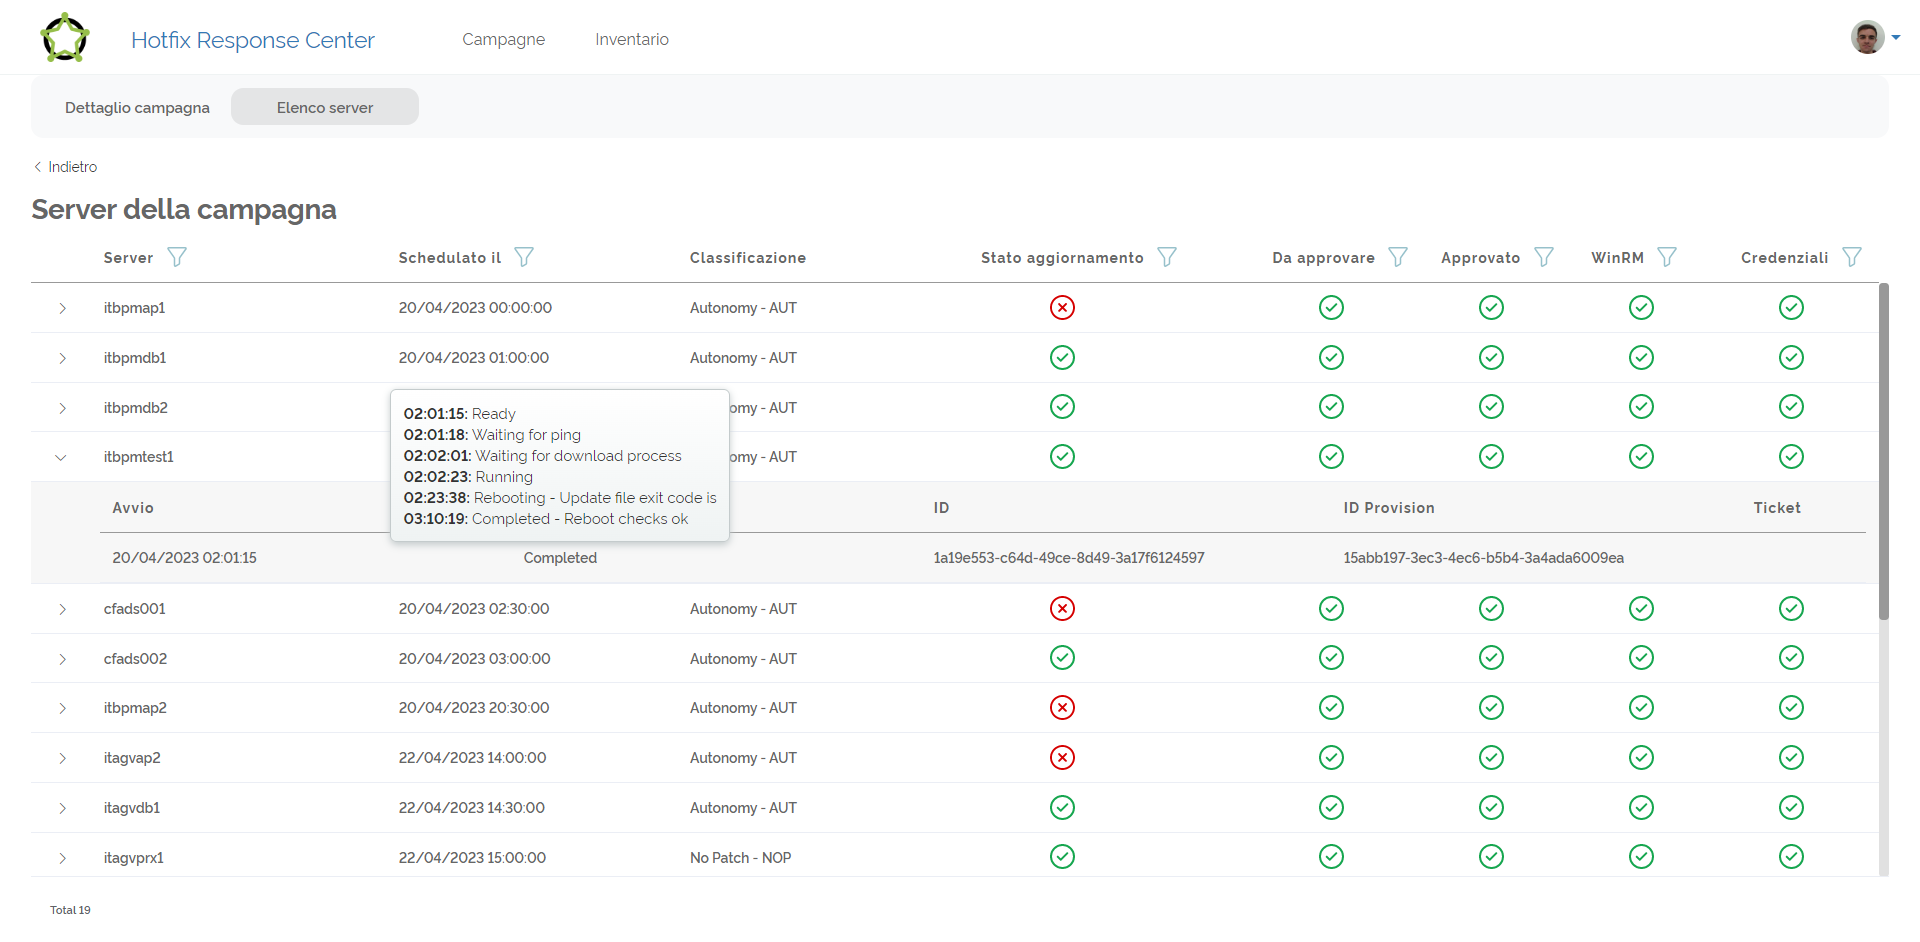
\includegraphics[width=0.98\textwidth]{imgs/ui/6_list_servers.png}}
    \caption{Elenco dei server della campagna}
    \label{fig:Elenco dei server della campagna}
\end{flushright}
\end{figure}

Attraverso la schermata “Elenco server”, è possibile visualizzare lo stato di 
aggiornamento di ogni singolo server. Tale stato può assumere quattro possibili 
valori: “Aggiornamento in attesa”, “Aggiornamento in corso”, “Completato” o “Fallito”.

Nel caso specifico di un aggiornamento fallito, è possibile utilizzare 
l'interfaccia del calendario per programmare manualmente una nuova data, al fine 
di tentare un aggiornamento automatico successivo. Tale funzionalità garantisce 
un'ulteriore opportunità per risolvere eventuali problemi e completare con 
successo l'aggiornamento del server interessato.\\

Nella maggior parte dei casi, l'aggiornamento risulta fallire a causa di server 
non raggiungibili o di credenziali di connessione non corrette. Quando ciò accade, 
è richiesto un intervento manuale per risolvere il problema prima di riprovare 
l'aggiornamento automatico. Per questo motivo si è deciso di lasciare all’operatore 
la decisione sulla scelta di una nuova data, per ritentare l'aggiornamento automatico.


\subsection{Conferma aggiornamento}
L’Hotfix Response Center è autonomamente in grado di riconoscere se 
l'aggiornamento è stato installato o meno sul server capendo anche se è 
necessario un riavvio per poterlo applicare correttamente.

In ogni caso, per verificare la corretta applicazione dell'aggiornamento di 
sicurezza applicato dalla campagna presa in analisi, è sufficiente collegarsi al 
server e verificare manualmente l’installazione lanciando il comando “Get-Hotfix” 
su una console Powershell con privilegi di amministratore.

\begin{figure}[H]
\begin{flushright}
    \centering
    \frame{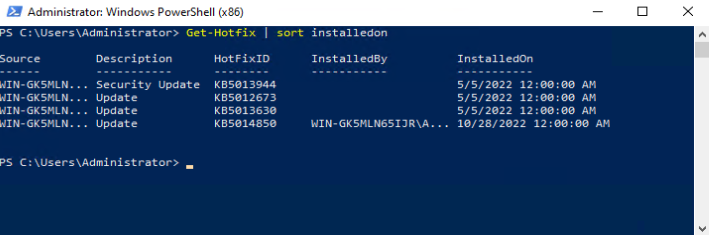
\includegraphics[width=0.98\textwidth]{imgs/ui/7_powershell_get_hotfix.png}}
    \caption{Console con il comando per verificare l'installazione dell'aggiornamento}
    \label{fig:Console con il comando per verificare l'installazione dell'aggiornamento}
\end{flushright}
\end{figure}

Nel server in questione possiamo notare che l'ultimo aggiornamento installato è
proprio l'aggiornamento cumulativo KB5014850 che conferma quindi l'installazione
remota e automatica dell'aggiornamento di sicurezza, attraverso la campagna di Hotfix.
